\documentclass[11pt,preprint, authoryear]{elsarticle}

\usepackage{lmodern}
%%%% My spacing
\usepackage{setspace}
\setstretch{1.2}
\DeclareMathSizes{12}{14}{10}{10}

% Wrap around which gives all figures included the [H] command, or places it "here". This can be tedious to code in Rmarkdown.
\usepackage{float}
\let\origfigure\figure
\let\endorigfigure\endfigure
\renewenvironment{figure}[1][2] {
    \expandafter\origfigure\expandafter[H]
} {
    \endorigfigure
}

\let\origtable\table
\let\endorigtable\endtable
\renewenvironment{table}[1][2] {
    \expandafter\origtable\expandafter[H]
} {
    \endorigtable
}


\usepackage{ifxetex,ifluatex}
\usepackage{fixltx2e} % provides \textsubscript
\ifnum 0\ifxetex 1\fi\ifluatex 1\fi=0 % if pdftex
  \usepackage[T1]{fontenc}
  \usepackage[utf8]{inputenc}
\else % if luatex or xelatex
  \ifxetex
    \usepackage{mathspec}
    \usepackage{xltxtra,xunicode}
  \else
    \usepackage{fontspec}
  \fi
  \defaultfontfeatures{Mapping=tex-text,Scale=MatchLowercase}
  \newcommand{\euro}{€}
\fi

\usepackage{amssymb, amsmath, amsthm, amsfonts}

\def\bibsection{\section*{References}} %%% Make "References" appear before bibliography


\usepackage[round]{natbib}

\usepackage{longtable}
\usepackage[margin=2.3cm,bottom=2cm,top=2.5cm, includefoot]{geometry}
\usepackage{fancyhdr}
\usepackage[bottom, hang, flushmargin]{footmisc}
\usepackage{graphicx}
\numberwithin{equation}{section}
\numberwithin{figure}{section}
\numberwithin{table}{section}
\setlength{\parindent}{0cm}
\setlength{\parskip}{1.3ex plus 0.5ex minus 0.3ex}
\usepackage{textcomp}
\renewcommand{\headrulewidth}{0pt}

\usepackage{array}
\newcolumntype{x}[1]{>{\centering\arraybackslash\hspace{0pt}}p{#1}}

%%%%  Remove the "preprint submitted to" part. Don't worry about this either, it just looks better without it:
\makeatletter
\def\ps@pprintTitle{%
  \let\@oddhead\@empty
  \let\@evenhead\@empty
  \let\@oddfoot\@empty
  \let\@evenfoot\@oddfoot
}
\makeatother

 \def\tightlist{} % This allows for subbullets!

\usepackage{hyperref}
\hypersetup{breaklinks=true,
            bookmarks=true,
            colorlinks=true,
            citecolor=blue,
            urlcolor=blue,
            linkcolor=blue,
            pdfborder={0 0 0}}


% The following packages allow huxtable to work:
\usepackage{siunitx}
\usepackage{multirow}
\usepackage{hhline}
\usepackage{calc}
\usepackage{tabularx}
\usepackage{booktabs}
\usepackage{caption}


\newenvironment{columns}[1][]{}{}

\newenvironment{column}[1]{\begin{minipage}{#1}\ignorespaces}{%
\end{minipage}
\ifhmode\unskip\fi
\aftergroup\useignorespacesandallpars}

\def\useignorespacesandallpars#1\ignorespaces\fi{%
#1\fi\ignorespacesandallpars}

\makeatletter
\def\ignorespacesandallpars{%
  \@ifnextchar\par
    {\expandafter\ignorespacesandallpars\@gobble}%
    {}%
}
\makeatother

\newenvironment{CSLReferences}[2]{%
}

\urlstyle{same}  % don't use monospace font for urls
\setlength{\parindent}{0pt}
\setlength{\parskip}{6pt plus 2pt minus 1pt}
\setlength{\emergencystretch}{3em}  % prevent overfull lines
\setcounter{secnumdepth}{5}

%%% Use protect on footnotes to avoid problems with footnotes in titles
\let\rmarkdownfootnote\footnote%
\def\footnote{\protect\rmarkdownfootnote}
\IfFileExists{upquote.sty}{\usepackage{upquote}}{}

%%% Include extra packages specified by user

%%% Hard setting column skips for reports - this ensures greater consistency and control over the length settings in the document.
%% page layout
%% paragraphs
\setlength{\baselineskip}{12pt plus 0pt minus 0pt}
\setlength{\parskip}{12pt plus 0pt minus 0pt}
\setlength{\parindent}{0pt plus 0pt minus 0pt}
%% floats
\setlength{\floatsep}{12pt plus 0 pt minus 0pt}
\setlength{\textfloatsep}{20pt plus 0pt minus 0pt}
\setlength{\intextsep}{14pt plus 0pt minus 0pt}
\setlength{\dbltextfloatsep}{20pt plus 0pt minus 0pt}
\setlength{\dblfloatsep}{14pt plus 0pt minus 0pt}
%% maths
\setlength{\abovedisplayskip}{12pt plus 0pt minus 0pt}
\setlength{\belowdisplayskip}{12pt plus 0pt minus 0pt}
%% lists
\setlength{\topsep}{10pt plus 0pt minus 0pt}
\setlength{\partopsep}{3pt plus 0pt minus 0pt}
\setlength{\itemsep}{5pt plus 0pt minus 0pt}
\setlength{\labelsep}{8mm plus 0mm minus 0mm}
\setlength{\parsep}{\the\parskip}
\setlength{\listparindent}{\the\parindent}
%% verbatim
\setlength{\fboxsep}{5pt plus 0pt minus 0pt}



\begin{document}



\begin{frontmatter}  %

\title{Predicting the best fantasy premier league team to pick per
gameweek}

% Set to FALSE if wanting to remove title (for submission)




\author[Add1]{Austin Byrne}
\ead{22582053@sun.ac.za}





\address[Add1]{Stellenbosch University, South Africa}


\begin{abstract}
\small{
Abstract to be written here. The abstract should not be too long and
should provide the reader with a good understanding what you are writing
about. Academic papers are not like novels where you keep the reader in
suspense. To be effective in getting others to read your paper, be as
open and concise about your findings here as possible. Ideally, upon
reading your abstract, the reader should feel he / she must read your
paper in entirety.
}
\end{abstract}

\vspace{1cm}





\vspace{0.5cm}

\end{frontmatter}

\setcounter{footnote}{0}



%________________________
% Header and Footers
%%%%%%%%%%%%%%%%%%%%%%%%%%%%%%%%%
\pagestyle{fancy}
\chead{}
\rhead{}
\lfoot{}
\rfoot{\footnotesize Page \thepage}
\lhead{}
%\rfoot{\footnotesize Page \thepage } % "e.g. Page 2"
\cfoot{}

%\setlength\headheight{30pt}
%%%%%%%%%%%%%%%%%%%%%%%%%%%%%%%%%
%________________________

\headsep 35pt % So that header does not go over title




\hypertarget{introduction}{%
\section{\texorpdfstring{Introduction
\label{Introduction}}{Introduction }}\label{introduction}}

\hypertarget{data-exploration}{%
\section{Data exploration}\label{data-exploration}}

\hypertarget{correlation-plot-between-player-attributes-and-total-points}{%
\subsection{Correlation plot between player attributes and total
points}\label{correlation-plot-between-player-attributes-and-total-points}}

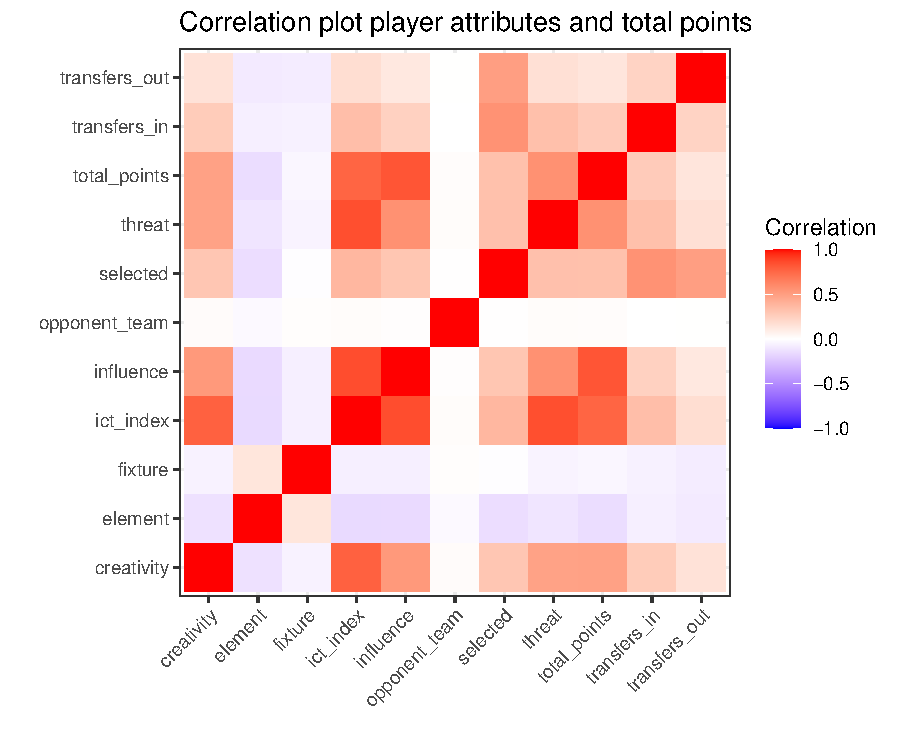
\includegraphics{Fantasy_premier_league_team_prediction_files/figure-latex/unnamed-chunk-2-1.pdf}

\hypertarget{correlation-plot-between-team-attributes-and-individual-player-points}{%
\subsection{Correlation plot between team attributes and individual
player
points}\label{correlation-plot-between-team-attributes-and-individual-player-points}}

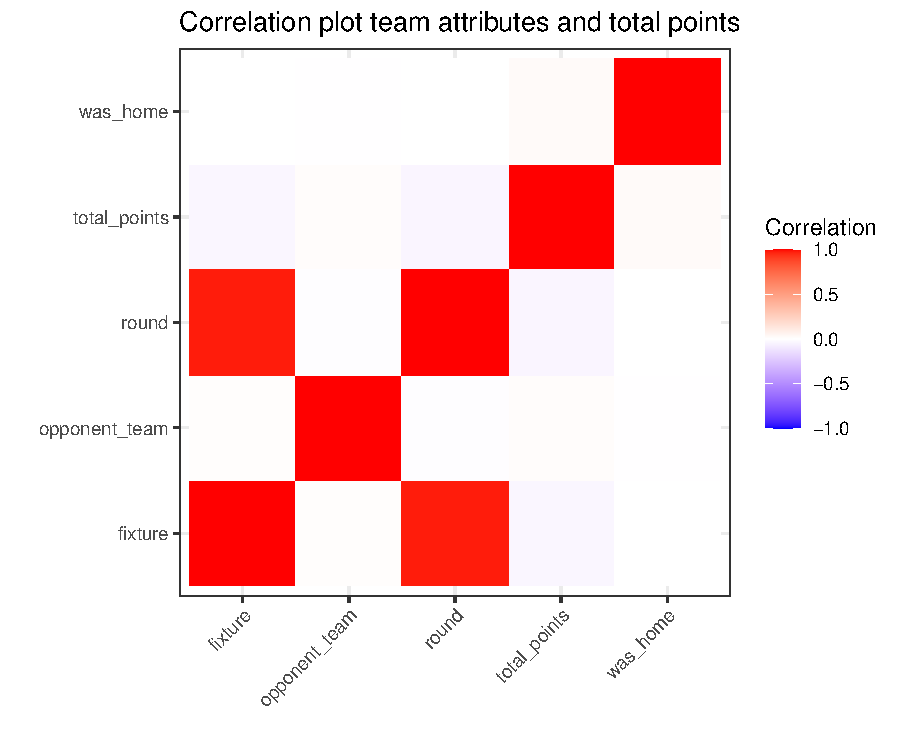
\includegraphics{Fantasy_premier_league_team_prediction_files/figure-latex/unnamed-chunk-3-1.pdf}

\hypertarget{plotting-the-average-points-scored-per-position-per-gameweek}{%
\subsection{Plotting the average points scored per position per
gameweek:}\label{plotting-the-average-points-scored-per-position-per-gameweek}}

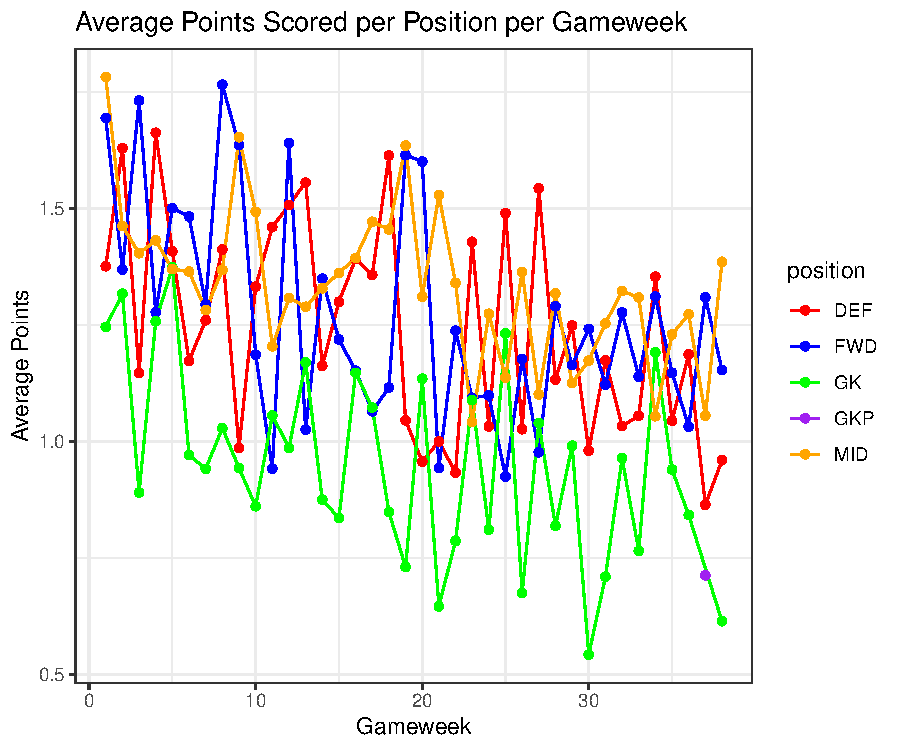
\includegraphics{Fantasy_premier_league_team_prediction_files/figure-latex/unnamed-chunk-4-1.pdf}

\hypertarget{now-plotting-the-average-points-per-postion-on-differetn-axis-and-plotting-the-overall-average-points-scored-per-postion.}{%
\subsection{Now plotting the average points per postion on differetn
axis and plotting the overall average points scored per
postion.}\label{now-plotting-the-average-points-per-postion-on-differetn-axis-and-plotting-the-overall-average-points-scored-per-postion.}}

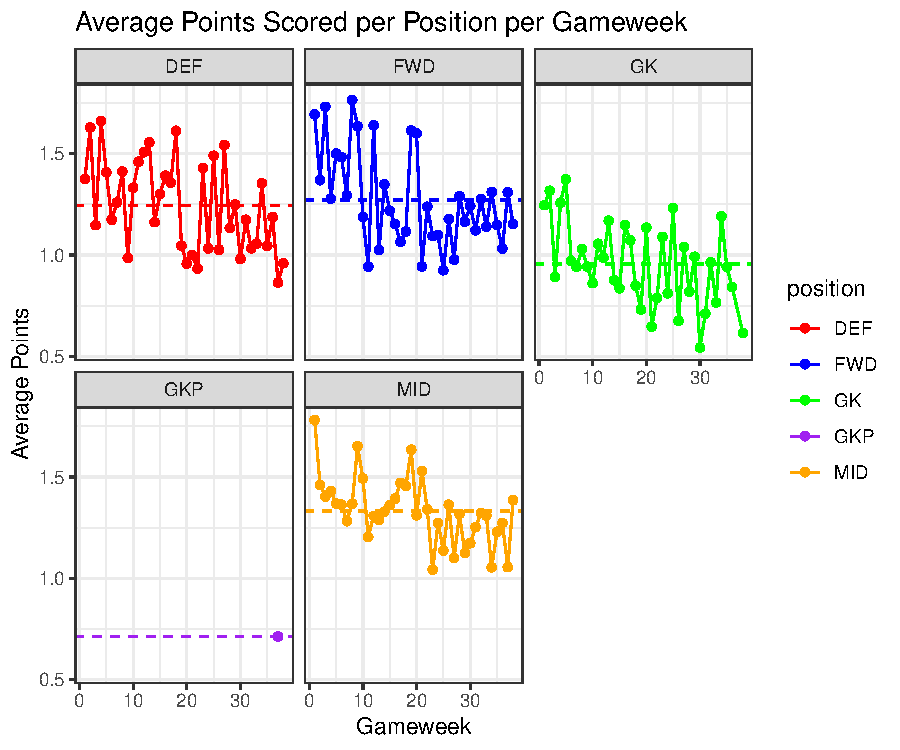
\includegraphics{Fantasy_premier_league_team_prediction_files/figure-latex/unnamed-chunk-5-1.pdf}

\hypertarget{scatter-plot-for-points-per-value}{%
\subsection{Scatter plot for points per
value:}\label{scatter-plot-for-points-per-value}}

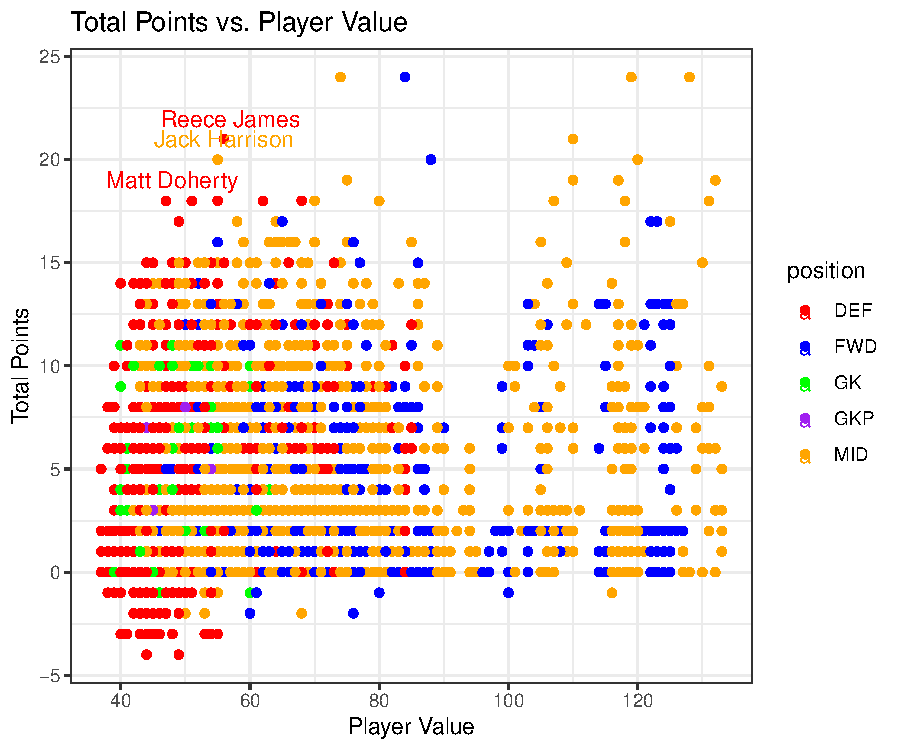
\includegraphics{Fantasy_premier_league_team_prediction_files/figure-latex/unnamed-chunk-6-1.pdf}

\hypertarget{minmean-and-max-points-per-team-for-a-gameweek}{%
\subsubsection{Min/mean and max points per team for a
gameweek:}\label{minmean-and-max-points-per-team-for-a-gameweek}}

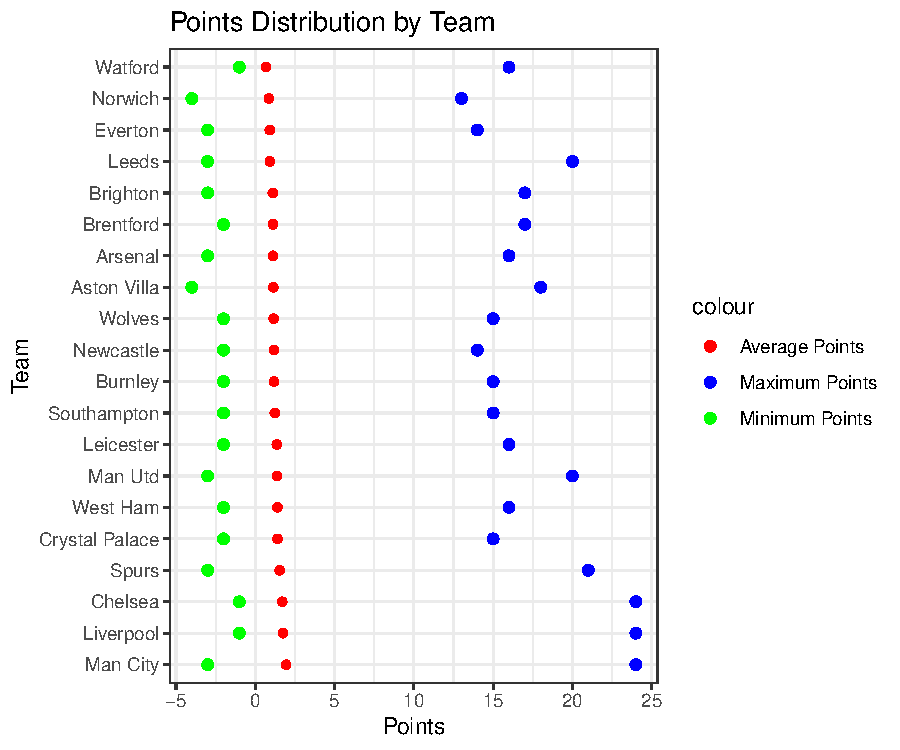
\includegraphics{Fantasy_premier_league_team_prediction_files/figure-latex/unnamed-chunk-7-1.pdf}

\hypertarget{machine-learning-model-using-random-forests}{%
\section{Machine learning model using Random
forests}\label{machine-learning-model-using-random-forests}}

\hypertarget{setup-process-of-machine-learning-model}{%
\subsection{setup process of machine learning
model}\label{setup-process-of-machine-learning-model}}

\hypertarget{creating-the-base-random-forests-model}{%
\subsubsection{Creating the base random forests
model}\label{creating-the-base-random-forests-model}}

\hypertarget{evaluating-the-performance-of-the-base-line-model}{%
\subsubsection{Evaluating the performance of the base line
model}\label{evaluating-the-performance-of-the-base-line-model}}

\begin{verbatim}
## [1] 0.3231536
\end{verbatim}

\begin{verbatim}
## [1] 0.6033058
\end{verbatim}

\hypertarget{hyper-parameter-tuning}{%
\subsection{Hyper parameter tuning}\label{hyper-parameter-tuning}}

\hypertarget{mtry-hyper-parameter-tuning}{%
\subsubsection{mtry hyper parameter
tuning}\label{mtry-hyper-parameter-tuning}}

\hypertarget{k-fold-hyper-parameter-tuning}{%
\subsubsection{k-fold Hyper parameter
tuning}\label{k-fold-hyper-parameter-tuning}}

\hypertarget{ntree-hyper-parameter-tuning}{%
\section{ntree hyper parameter
tuning}\label{ntree-hyper-parameter-tuning}}

\hypertarget{best-model-after-hyper-parameter-tuning}{%
\subsection{Best model after hyper parameter
tuning}\label{best-model-after-hyper-parameter-tuning}}

\hypertarget{evaluating-the-performance-of-the-tuned-model}{%
\subsection{Evaluating the performance of the tuned
model}\label{evaluating-the-performance-of-the-tuned-model}}

\begin{verbatim}
## [1] 0.3210782
\end{verbatim}

\begin{verbatim}
## [1] 0.6019206
\end{verbatim}

\hypertarget{time-for-predictions}{%
\section{Time for predictions}\label{time-for-predictions}}

\newpage

\hypertarget{references}{%
\section*{References}\label{references}}
\addcontentsline{toc}{section}{References}

\hypertarget{refs}{}
\begin{CSLReferences}{0}{0}
\end{CSLReferences}

\hypertarget{appendix}{%
\section*{Appendix}\label{appendix}}
\addcontentsline{toc}{section}{Appendix}

\hypertarget{appendix-a}{%
\subsection*{Appendix A}\label{appendix-a}}
\addcontentsline{toc}{subsection}{Appendix A}

Some appendix information here

\hypertarget{appendix-b}{%
\subsection*{Appendix B}\label{appendix-b}}
\addcontentsline{toc}{subsection}{Appendix B}

\bibliography{Tex/ref}





\end{document}
